In this section, we briefly summarize the SDC formulation for IVPs and
then extend SDC to an integro-differential equation that governs
vesicle dynamics.  We first discuss the theory of SDC and then describe
its numerical implementation in Section~\ref{s:numerics}.

%%%%%%%%%%%%%%%%%%%%%%%%%%%%%%%%%%%%%%%%%%%%%%%%%%%%%%%%%%%%%%%%%%%%%%%%
\subsection{Spectral Deferred Correction}
In its original development~\cite{dut:gre:rok2000}, SDC iteratively
constructed a high-order solution of the IVP
\begin{align}
  \frac{d\xx}{dt} = f(\xx,t), \quad t \in [0,T],
  \quad \xx(0) = \xx_{0}. 
\label{e:ivp}
\end{align}
While classical deferred correction methods discretize the time
derivative in~\eqref{e:ivp}, SDC uses a Picard integral to avoid
unstable numerical differentiation.  Equation~\eqref{e:ivp} is
reformulated as
\begin{align}
  \xx(t) = \xx_{0} + \int_{0}^{t} f(\xx,\tau) d\tau, \quad t \in [0,T].
\label{e:picardIVP}
\end{align}
A time stepping scheme is applied to compute a numerical solution at $p$
quadrature points in $[t_{m},t_{m+1}]$.  By interpolating at these
quadrature points, a provisional solution $\txx{}(t)$ is generated.
Given this provisional solution $\txx{}(t)$ of~\eqref{e:picardIVP}, the
residual is defined as
\begin{align}
  \rr(t;\txx{}) = \xx(t_{m}) - \txx{}(t) + 
    \int_{t_{m}}^{t} f(\txx{},\tau) d\tau, 
    \quad t \in [t_{m},t_{m+1}].
  \label{e:picardResidual}
\end{align}
The provisional solution at the $p$ quadrature points is then used to
approximate the integral in~\eqref{e:picardResidual} with
$p^{th}$-order accuracy.  The error $\ee = \xx - \txx{}$ satisfies
\begin{align}
  \ee(t) = \rr(t;\txx{}) + \int_{t_{m}}^{t} 
      (f(\txx{} + \ee,\tau) - f(\txx,\tau)) d\tau, \quad
      t \in [t_{m},t_{m+1}],
  \label{e:picardCorrect}
\end{align}
and an approximation $\tilde{\ee}$ of $\ee$ is computed, generally
using the same numerical method used to compute $\txx{}$.  Finally, the
provisional solution is updated to $\txx{} + \tilde{\ee}$ and the
procedure is repeated as many times as desired.  The process of forming
the residual $\rr$, approximating the error $\ee$, and updating the
provisional solution is referred to as an SDC iteration or sweep.  We
note that a time stepping scheme forms a discrete provisional solution
which does not have to be interpolated; instead, one forms discrete
values at quadrature points which are then used to approximate the
residual $\rr$.

The accuracy of SDC depends on the discretization
of~\eqref{e:picardIVP} and~\eqref{e:picardCorrect} and the accuracy of
the quadrature rule used to estimate $\rr(t;\txx{})$.  An abstract
error analysis for applying deferred correction methods to the operator
equation $F(y)=0$ has been performed
in~\cite{boh:ste1984,lin1980,ske1982,ste1973}.  In~\cite{han:str2011},
this abstract framework was applied to~\eqref{e:ivp} and the main
result is stated in Theorem 4.2.  Here we formulate the result in terms
of first-order corrections, which we will be using.
\begin{proposition}
\label{pro:convergence}
Let $\xx$ be the unique solution of~\eqref{e:ivp}, and $\txx{}$ be an
order $k$ approximation of $\xx$ formed with a stable time integrator
meaning that
\begin{align*}
  \|\txx{}(T) - \xx(T)\| = \mathcal{O}(\Delta t^{k}),
\end{align*}
where the constant depends only on the derivatives of $f$ and on $T$,
but not on $\Delta t$.  Assume the residual~\eqref{e:picardResidual} is
computed exactly.  If the exact error $\ee$
satisfying~\eqref{e:picardCorrect} is approximated with a first-order
solution $\tee{}$, then
\begin{align*}
  \|\tee{}(T) + \txx{}(T) - \xx(T)\| = \mathcal{O}(\Delta t^{k+1}).
\end{align*}
However, since $\rr$ is approximated with a quadrature rule,
the asymptotic error is
\begin{align*}
  \|\tee{}(T) + \txx{}(T) - \xx(T)\| = \bigO(\Delta t^{\min(k+1,\ell)}),
\end{align*}
where $\ell$ is the quadrature's order of accuracy.
\end{proposition}
%\begin{theorem} 
%\label{thm:convergence}
%Let $f \in C^{\infty}$ have bounded derivatives, and $\xx$ be the unique
%solution of~\eqref{e:ivp}.  Suppose that the time integrator $\phi$ is
%stable.  That is, there exists some $S > 0$ which only depends on $f$
%and $T$, such that for all $\yy, \zz \in \RR^{m}$,
%\begin{align*}
%  \|\yy - \zz\| \leq S\|\phi_{m}(\yy) - \phi_{m}(\zz)\|.
%\end{align*}
%Moreover, suppose that $\phi_{m}$ is of order $k$ meaning that
%$\phi_{m}(\xx) = \mathcal{O}(\Delta t^{k})$, where $\Delta t = T/m$.
%Suppose that a numerical solution $\txx{}$ of $\xx$ satisfies
%\begin{align*}
%  \|\txx{}(T) - \xx(T)\| \leq C \Delta t^{\ell},
%\end{align*}
%where $C$ depends only on the derivatives of $f$ and on $T$, but not on
%$m$.  Assuming the residual $\rr$ is computed exactly, if $\tee{}$ is
%formed with the order $k$ time integrator $\phi$ to approximate $\ee$,
%then
%\begin{align*}
%  \|\tee{}(T) + \txx{}(T) - \xx(T)\| \leq C \Delta t^{\ell+k}.
%\end{align*}
%However, since $\rr$ is approximated with a $p^{th}$-order quadrature,
%the asymptotic error is
%\begin{align*}
%  \|\tee{}(T) + \txx{}(T) - \xx(T)\| = \bigO(\Delta t^{\min(\ell+k,p)}).
%\end{align*}
%\end{theorem}

Proposition~\ref{pro:convergence} tells us that by estimating the error
$\ee$ with a first-order method, which is the only order we will
consider, the order of accuracy is increased by one, with the constraint
that this convergence is limited by the accuracy of the quadrature rule
for approximating~\eqref{e:picardResidual}.  However, the theorem states
nothing about the stability of SDC.  In~\cite{dut:gre:rok2000}, the
authors consider three discretizations of~\eqref{e:picardIVP}
and~\eqref{e:picardCorrect}: fully explicit, fully implicit, and linear
combinations of the two.  We do not consider explicit methods since the
governing equations are stiff.  The other two methods could be used for
vesicle suspensions, but both would require solving non-linear
equations.

We have successfully used a variant of IMEX methods for vesicle
suspensions~\cite{qua:bir2014b, rah:vee:bir2010, vee:gue:zor:bir2009},
and we couple these methods with SDC in this work.  IMEX
methods~\cite{asc:ruu:wet1995} are a family of time integrators that
treat some terms (generally, linear) implicitly and other terms
explicitly.  IMEX methods for additive splittings $\dot{\xx}(t) =
F_{\mathrm{EXPLICIT}}(\xx,t) + F_{\mathrm{IMPLICIT}}(\xx,t) =
F_{E}(\xx,t) + F_{I}(\xx,t)$ of~\eqref{e:ivp} were first applied to SDC
by Minion~\cite{min2003}.  We summarize the numerical results
from~\cite{min2003} since their behaviour resembles results that we
will observe.  First, the Van der Pol oscillator is considered in a
non-stiff, mildly stiff, and stiff regime, and the number of SDC
iterations ranges from two to six.  In the non-stiff regime, the error
behaves according to Proposition~\ref{pro:convergence}.  In the mildly
stiff case, the correct asymptotic result is observed, but not until
$\Delta t$ is much smaller.  In the stiff regime, the convergence
behaviour differs considerably from the formal error.  This behaviour
is attributed to order reduction which is further analyzed.  The author
proceeds to claim that ``the correct asymptotic convergence rates would
be observed given sufficiently small $\Delta t$; however, this is not
the relevant issue in most applications".

An alternative interpretation of SDC which is often useful is as an
iterative method that is converging to the solution of the
fully-implicit Gaussian collocation scheme of~\eqref{e:picardIVP}.  By
using this interpretation, Krylov deferred correction
methods~\cite{hua:jia:min2006, jia:hua2008, bu:hua:min2009,
bu:hua:min2012, hua:jia:min2007} can be applied, the stability and
convergence properties of SDC can analyzed and improved~\cite{wei2013},
and inexact and multilevel approximations can be
made~\cite{spe:rup:emm:bol:kra2014, emm:min2012,
min:spe:bol:emm:rup2015, spe:rup:emm:min:bol:kra2014,
spe:rup:min:emm:kra2014}.  These methods have been shown to accelerate
SDC convergence.  However, in this first work on applying SDC to
vesicle suspensions, we focus on using the simplest algorithm: we apply
a preselected number of SDC iterations to a set of quadrature points
which remain fixed at all the SDC iterations.

%%%%%%%%%%%%%%%%%%%%%%%%%%%%%%%%%%%%%%%%%%%%%%%%%%%%%%%%%%%%%%%%%%%%%%%%
\subsection{SDC for Vesicle Suspensions}

Let $\{\gamma_{j}\}_{j=1}^{M}$ be a collection of vesicles
parameterized by $\xx_{j}$ and with tension $\sigma_{j}$
(Figure~\ref{f:schematics}).  We use the integro-differential equation
derived in~\cite{vee:gue:zor:bir2009}.  It expresses the balance of the
bending and tension forces of the vesicle with the stress jump of the
fluid across the vesicle membrane and is augmented by a constraint to
enforce the inextensibility condition. In detail, the equations that
govern the evolution of the vesicle suspensions is an equation for the
velocity of the interface~\eqref{e:diffEqn} and the vesicle surface
inextensibility condition~\eqref{e:inextens}. The key term in these two
equations is $\vv(\xx_{j};\xx_{k})$---the velocity of vesicle $j$ due
to the hydrodynamic forces from vesicle $k$. This term is given by
\begin{align}
  \vv(\xx_{j};\xx_{k}) = \vv_{\infty}(\xx_{j})\delta_{j,k} + \SS(\xx_{j},\xx_{k})
    (-\BB(\xx_{k})(\xx_{k}) + \TT(\xx_{k})(\sigma_{k})),
  \label{e:vesDynamics}
\end{align}
where $\delta_{j,k}$ is the Kronecker delta function,
%\begin{align*}
%  &s = \|\xx'\|, \quad \quad \rho = \|\xx - \yy\|, \\
%  &\SS(\xx_{j},\xx_{k})(\ff) = \frac{1}{4\pi}\int_{\gamma_{k}} \left(
%    -\log \rho + \frac{(\xx - \yy) \otimes (\xx - \yy)}{\rho^{2}} \right)
%    \ff(\yy) ds_{\yy}, \quad \xx \in \gamma_{j}, \\
%  &\BB(\xx)(\ff) = \frac{d^{4}\ff}{ds^{4}}, \\ 
%  &\TT(\xx)(\sigma) =
%    \frac{d}{ds}\left(\sigma\frac{d\xx}{ds}\right),
%\end{align*}
\begin{align*}
  &\SS(\xx_{j},\xx_{k})(\ff) = \frac{1}{4\pi}\int_{\gamma_{k}} \left(
    -\log \rho + \frac{(\xx_{j} - \xx_{k}) \otimes (\xx_{j} - \xx_{k})}{\rho^{2}} \right)
    \ff(\xx_{k}) ds_{k}, \\
  &\rho = \|\xx_{j} - \xx_{k}\|, \\
  &\BB(\xx_{k})(\ff) = \frac{d^{4}\ff}{ds_{k}^{4}}, \\ 
  &\TT(\xx_{k})(\sigma_{k}) =
    \frac{d}{ds_{k}}\left(\sigma_{k}\frac{d\xx_{k}}{ds_{k}}\right),
\end{align*}
$s_{k}$ is the arclength of $\gamma_{k}$, and $\vv_{\infty}$ is the
background velocity (unconfined flows) or the velocity due to solid
walls (confined flows).  In the case of confined flows, we use the
double-layer potential of an unknown density function $\eeta$ defined on
the boundary of the solid walls.  The extra equation comes from a
non-slip boundary condition on the solid walls and the details are
presented in~\cite{rah:vee:bir2010}.  We point out that $\vv$ is not
symmetric, meaning that $\vv(\xx_{j};\xx_{k}) \neq \vv(\xx_{k};\xx_{j})$
for all $j \neq k$, and $\SS$, $\BB$, $\TT$ are all linear in their
second argument.

The notation we are using is chosen so that terms such as
$\BB(\xx_{k}^{m+1})(\xx_{k}^{m+1})$ can be approximated as
\begin{align*}
  \BB(\xx_{k}^{m})(\xx_{k}^{m+1}) = 
    \frac{d^{4}}{ds_{k}^{4}} \xx_{k}^{m+1}.
\end{align*}
The tension $\sigma_{j}$ acts as a Lagrange multiplier to satisfy the
inextensibility constraint
\begin{align}
  \Div(\xx_{j})\left(\sum_{k=1}^{M}\vv(\xx_{j};\xx_{k})\right) = 0,
  \label{e:inextens}
\end{align}
where
\begin{align*}
  \Div(\xx_{j})(\ff) = \frac{d\xx_{j}}{ds_{j}} 
      \cdot \frac{d\ff}{ds_{j}},
\end{align*}
which is also linear in its second argument.
Equation~\eqref{e:inextens} can be eliminated using the Schur
complement of the tension to write $\sigma_{j}$ in terms of the
positions
$\xx_{k}$, $k=1,\ldots,M$.  Then, the vesicle
velocity~\eqref{e:vesDynamics} can be written entirely in terms of
$\xx_{j}$ and $\xx_{k}$, and the no-slip boundary condition of vesicle
$j$ gives
\begin{align}
  \frac{d\xx_{j}}{dt} = \sum_{k=1}^{M}\vv(\xx_{j};\xx_{k}), \quad
  j=1,\ldots,M.
  \label{e:diffEqn}
\end{align}
The formulation~\eqref{e:diffEqn} is easiest to present our numerical
methods, but we in fact do not eliminate the tension in our
implementation.  The resulting changes to the SDC formulation are
presented in Appendix~\ref{a:appendix1}.

\begin{figure}[htp]
\begin{center}
  \begin{tabular}{cc}
  \ifTikz
  \scalebox{0.9}{%\documentclass[11pt]{article}
%\usepackage{tikz,pgfplots}
%\begin{document}
%
%
%
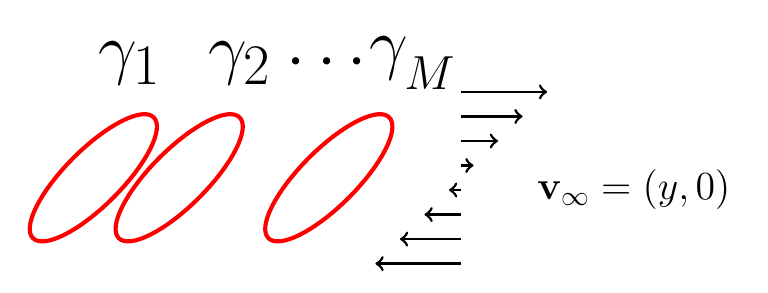
\begin{tikzpicture}[scale=1.0]

\begin{axis}[
  xmin = -3,
  xmax = 19,
  ymin = -6,
  ymax = 6,
  axis equal = true,
  hide axis,
  ]

\addplot [mark=none,red,line width=1.5] table{
2.4625e+00 2.4625e+00
2.3710e+00 2.5302e+00
2.2567e+00 2.5736e+00
2.1207e+00 2.5922e+00
1.9642e+00 2.5859e+00
1.7889e+00 2.5546e+00
1.5963e+00 2.4987e+00
1.3883e+00 2.4188e+00
1.1669e+00 2.3155e+00
9.3436e-01 2.1900e+00
6.9278e-01 2.0434e+00
4.4453e-01 1.8771e+00
1.9199e-01 1.6927e+00
-6.2390e-02 1.4920e+00
-3.1617e-01 1.2770e+00
-5.6691e-01 1.0496e+00
-8.1219e-01 8.1219e-01
-1.0496e+00 5.6691e-01
-1.2770e+00 3.1617e-01
-1.4920e+00 6.2390e-02
-1.6927e+00 -1.9199e-01
-1.8771e+00 -4.4453e-01
-2.0434e+00 -6.9278e-01
-2.1900e+00 -9.3436e-01
-2.3155e+00 -1.1669e+00
-2.4188e+00 -1.3883e+00
-2.4987e+00 -1.5963e+00
-2.5546e+00 -1.7889e+00
-2.5859e+00 -1.9642e+00
-2.5922e+00 -2.1207e+00
-2.5736e+00 -2.2567e+00
-2.5302e+00 -2.3710e+00
-2.4625e+00 -2.4625e+00
-2.3710e+00 -2.5302e+00
-2.2567e+00 -2.5736e+00
-2.1207e+00 -2.5922e+00
-1.9642e+00 -2.5859e+00
-1.7889e+00 -2.5546e+00
-1.5963e+00 -2.4987e+00
-1.3883e+00 -2.4188e+00
-1.1669e+00 -2.3155e+00
-9.3436e-01 -2.1900e+00
-6.9278e-01 -2.0434e+00
-4.4453e-01 -1.8771e+00
-1.9199e-01 -1.6927e+00
6.2390e-02 -1.4920e+00
3.1617e-01 -1.2770e+00
5.6691e-01 -1.0496e+00
8.1219e-01 -8.1219e-01
1.0496e+00 -5.6691e-01
1.2770e+00 -3.1617e-01
1.4920e+00 -6.2390e-02
1.6927e+00 1.9199e-01
1.8771e+00 4.4453e-01
2.0434e+00 6.9278e-01
2.1900e+00 9.3436e-01
2.3155e+00 1.1669e+00
2.4188e+00 1.3883e+00
2.4987e+00 1.5963e+00
2.5546e+00 1.7889e+00
2.5859e+00 1.9642e+00
2.5922e+00 2.1207e+00
2.5736e+00 2.2567e+00
2.5302e+00 2.3710e+00
2.4625e+00 2.4625e+00
};

\addplot [mark=none,red,line width=1.5] table{
5.9625e+00 2.4625e+00
5.8710e+00 2.5302e+00
5.7567e+00 2.5736e+00
5.6207e+00 2.5922e+00
5.4642e+00 2.5859e+00
5.2889e+00 2.5546e+00
5.0963e+00 2.4987e+00
4.8883e+00 2.4188e+00
4.6669e+00 2.3155e+00
4.4344e+00 2.1900e+00
4.1928e+00 2.0434e+00
3.9445e+00 1.8771e+00
3.6920e+00 1.6927e+00
3.4376e+00 1.4920e+00
3.1838e+00 1.2770e+00
2.9331e+00 1.0496e+00
2.6878e+00 8.1219e-01
2.4504e+00 5.6691e-01
2.2230e+00 3.1617e-01
2.0080e+00 6.2390e-02
1.8073e+00 -1.9199e-01
1.6229e+00 -4.4453e-01
1.4566e+00 -6.9278e-01
1.3100e+00 -9.3436e-01
1.1845e+00 -1.1669e+00
1.0812e+00 -1.3883e+00
1.0013e+00 -1.5963e+00
9.4541e-01 -1.7889e+00
9.1414e-01 -1.9642e+00
9.0778e-01 -2.1207e+00
9.2638e-01 -2.2567e+00
9.6976e-01 -2.3710e+00
1.0375e+00 -2.4625e+00
1.1290e+00 -2.5302e+00
1.2433e+00 -2.5736e+00
1.3793e+00 -2.5922e+00
1.5358e+00 -2.5859e+00
1.7111e+00 -2.5546e+00
1.9037e+00 -2.4987e+00
2.1117e+00 -2.4188e+00
2.3331e+00 -2.3155e+00
2.5656e+00 -2.1900e+00
2.8072e+00 -2.0434e+00
3.0555e+00 -1.8771e+00
3.3080e+00 -1.6927e+00
3.5624e+00 -1.4920e+00
3.8162e+00 -1.2770e+00
4.0669e+00 -1.0496e+00
4.3122e+00 -8.1219e-01
4.5496e+00 -5.6691e-01
4.7770e+00 -3.1617e-01
4.9920e+00 -6.2390e-02
5.1927e+00 1.9199e-01
5.3771e+00 4.4453e-01
5.5434e+00 6.9278e-01
5.6900e+00 9.3436e-01
5.8155e+00 1.1669e+00
5.9188e+00 1.3883e+00
5.9987e+00 1.5963e+00
6.0546e+00 1.7889e+00
6.0859e+00 1.9642e+00
6.0922e+00 2.1207e+00
6.0736e+00 2.2567e+00
6.0302e+00 2.3710e+00
5.9625e+00 2.4625e+00
};

\addplot [mark=none,red,line width=1.5] table{
1.2062e+01 2.4625e+00
1.1971e+01 2.5302e+00
1.1857e+01 2.5736e+00
1.1721e+01 2.5922e+00
1.1564e+01 2.5859e+00
1.1389e+01 2.5546e+00
1.1196e+01 2.4987e+00
1.0988e+01 2.4188e+00
1.0767e+01 2.3155e+00
1.0534e+01 2.1900e+00
1.0293e+01 2.0434e+00
1.0045e+01 1.8771e+00
9.7920e+00 1.6927e+00
9.5376e+00 1.4920e+00
9.2838e+00 1.2770e+00
9.0331e+00 1.0496e+00
8.7878e+00 8.1219e-01
8.5504e+00 5.6691e-01
8.3230e+00 3.1617e-01
8.1080e+00 6.2390e-02
7.9073e+00 -1.9199e-01
7.7229e+00 -4.4453e-01
7.5566e+00 -6.9278e-01
7.4100e+00 -9.3436e-01
7.2845e+00 -1.1669e+00
7.1812e+00 -1.3883e+00
7.1013e+00 -1.5963e+00
7.0454e+00 -1.7889e+00
7.0141e+00 -1.9642e+00
7.0078e+00 -2.1207e+00
7.0264e+00 -2.2567e+00
7.0698e+00 -2.3710e+00
7.1375e+00 -2.4625e+00
7.2290e+00 -2.5302e+00
7.3433e+00 -2.5736e+00
7.4793e+00 -2.5922e+00
7.6358e+00 -2.5859e+00
7.8111e+00 -2.5546e+00
8.0037e+00 -2.4987e+00
8.2117e+00 -2.4188e+00
8.4331e+00 -2.3155e+00
8.6656e+00 -2.1900e+00
8.9072e+00 -2.0434e+00
9.1555e+00 -1.8771e+00
9.4080e+00 -1.6927e+00
9.6624e+00 -1.4920e+00
9.9162e+00 -1.2770e+00
1.0167e+01 -1.0496e+00
1.0412e+01 -8.1219e-01
1.0650e+01 -5.6691e-01
1.0877e+01 -3.1617e-01
1.1092e+01 -6.2390e-02
1.1293e+01 1.9199e-01
1.1477e+01 4.4453e-01
1.1643e+01 6.9278e-01
1.1790e+01 9.3436e-01
1.1916e+01 1.1669e+00
1.2019e+01 1.3883e+00
1.2099e+01 1.5963e+00
1.2155e+01 1.7889e+00
1.2186e+01 1.9642e+00
1.2192e+01 2.1207e+00
1.2174e+01 2.2567e+00
1.2130e+01 2.3710e+00
1.2062e+01 2.4625e+00
};

  \foreach \y in {-3.5,-2.5,-1.5,-0.5,0.5,1.5,2.5,3.5}
     \addplot[color=black,line width = 1.0pt,solid,->]
       plot coordinates{(15,\y)(15+\y,\y)};


\end{axis}

%\draw[gray,thin] (0,1) grid +(8,4);
\node[font = \Huge] at (1.4,4.3) {$\gamma_{1}$};
\node[font = \Huge] at (2.8,4.3) {$\gamma_{2}$};
\node[font = \Huge] at (3.9,4.3) {$\cdots$};
\node[font = \Huge] at (5.0,4.3) {$\gamma_{_{M}}$};

\node[font = \Large] at (7.8,2.7) {$\mathbf{v}_{\infty} = (y,0)$};

\end{tikzpicture}

%\end{document}
} & 
  \scalebox{0.9}{%\documentclass[11pt]{article}
%\usepackage{tikz,pgfplots}
%\begin{document}
%
%
%
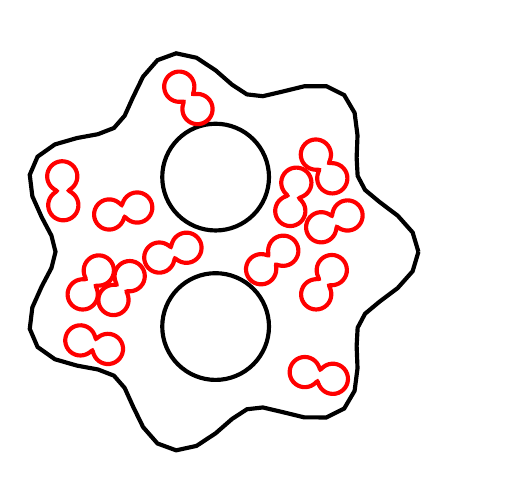
\begin{tikzpicture}[scale=1.0]

\begin{axis}[
  xmin = -21,
  xmax = 21,
  ymin = -21,
  ymax = 21,
  axis equal = true,
  hide axis,
  ]

\addplot [mark=none,black,line width=1.5] table{
1.9000e+01 0.0000e+00
1.8457e+01 1.8178e+00
1.7056e+01 3.3927e+00
1.5366e+01 4.6612e+00
1.3999e+01 5.7985e+00
1.3305e+01 7.1115e+00
1.3211e+01 8.8274e+00
1.3293e+01 1.0909e+01
1.3021e+01 1.3021e+01
1.2047e+01 1.4680e+01
1.0369e+01 1.5518e+01
8.2874e+00 1.5505e+01
6.2127e+00 1.4999e+01
4.4228e+00 1.4580e+01
2.9339e+00 1.4749e+01
1.5419e+00 1.5655e+01
1.0409e-15 1.7000e+01
-1.7907e+00 1.8181e+01
-3.6992e+00 1.8597e+01
-5.4469e+00 1.7956e+01
-6.7985e+00 1.6413e+01
-7.7401e+00 1.4481e+01
-8.5208e+00 1.2752e+01
-9.5220e+00 1.1603e+01
-1.1021e+01 1.1021e+01
-1.2990e+01 1.0660e+01
-1.5059e+01 1.0062e+01
-1.6681e+01 8.9159e+00
-1.7413e+01 7.2127e+00
-1.7170e+01 5.2085e+00
-1.6291e+01 3.2404e+00
-1.5380e+01 1.5148e+00
-1.5000e+01 1.8370e-15
-1.5380e+01 -1.5148e+00
-1.6291e+01 -3.2404e+00
-1.7170e+01 -5.2085e+00
-1.7413e+01 -7.2127e+00
-1.6681e+01 -8.9159e+00
-1.5059e+01 -1.0062e+01
-1.2990e+01 -1.0660e+01
-1.1021e+01 -1.1021e+01
-9.5220e+00 -1.1603e+01
-8.5208e+00 -1.2752e+01
-7.7401e+00 -1.4481e+01
-6.7985e+00 -1.6413e+01
-5.4469e+00 -1.7956e+01
-3.6992e+00 -1.8597e+01
-1.7907e+00 -1.8181e+01
-3.1228e-15 -1.7000e+01
1.5419e+00 -1.5655e+01
2.9339e+00 -1.4749e+01
4.4228e+00 -1.4580e+01
6.2127e+00 -1.4999e+01
8.2874e+00 -1.5505e+01
1.0369e+01 -1.5518e+01
1.2047e+01 -1.4680e+01
1.3021e+01 -1.3021e+01
1.3293e+01 -1.0909e+01
1.3211e+01 -8.8274e+00
1.3305e+01 -7.1115e+00
1.3999e+01 -5.7985e+00
1.5366e+01 -4.6612e+00
1.7056e+01 -3.3927e+00
1.8457e+01 -1.8178e+00
1.9000e+01 0.0000e+00
};

\addplot [mark=none,black,line width=1.5] table{
5.0000e+00 -7.0000e+00
4.9759e+00 -7.4901e+00
4.9039e+00 -7.9755e+00
4.7847e+00 -8.4514e+00
4.6194e+00 -8.9134e+00
4.4096e+00 -9.3570e+00
4.1573e+00 -9.7779e+00
3.8651e+00 -1.0172e+01
3.5355e+00 -1.0536e+01
3.1720e+00 -1.0865e+01
2.7779e+00 -1.1157e+01
2.3570e+00 -1.1410e+01
1.9134e+00 -1.1619e+01
1.4514e+00 -1.1785e+01
9.7545e-01 -1.1904e+01
4.9009e-01 -1.1976e+01
3.0616e-16 -1.2000e+01
-4.9009e-01 -1.1976e+01
-9.7545e-01 -1.1904e+01
-1.4514e+00 -1.1785e+01
-1.9134e+00 -1.1619e+01
-2.3570e+00 -1.1410e+01
-2.7779e+00 -1.1157e+01
-3.1720e+00 -1.0865e+01
-3.5355e+00 -1.0536e+01
-3.8651e+00 -1.0172e+01
-4.1573e+00 -9.7779e+00
-4.4096e+00 -9.3570e+00
-4.6194e+00 -8.9134e+00
-4.7847e+00 -8.4514e+00
-4.9039e+00 -7.9755e+00
-4.9759e+00 -7.4901e+00
-5.0000e+00 -7.0000e+00
-4.9759e+00 -6.5099e+00
-4.9039e+00 -6.0245e+00
-4.7847e+00 -5.5486e+00
-4.6194e+00 -5.0866e+00
-4.4096e+00 -4.6430e+00
-4.1573e+00 -4.2221e+00
-3.8651e+00 -3.8280e+00
-3.5355e+00 -3.4645e+00
-3.1720e+00 -3.1349e+00
-2.7779e+00 -2.8427e+00
-2.3570e+00 -2.5904e+00
-1.9134e+00 -2.3806e+00
-1.4514e+00 -2.2153e+00
-9.7545e-01 -2.0961e+00
-4.9009e-01 -2.0241e+00
-9.1849e-16 -2.0000e+00
4.9009e-01 -2.0241e+00
9.7545e-01 -2.0961e+00
1.4514e+00 -2.2153e+00
1.9134e+00 -2.3806e+00
2.3570e+00 -2.5904e+00
2.7779e+00 -2.8427e+00
3.1720e+00 -3.1349e+00
3.5355e+00 -3.4645e+00
3.8651e+00 -3.8280e+00
4.1573e+00 -4.2221e+00
4.4096e+00 -4.6430e+00
4.6194e+00 -5.0866e+00
4.7847e+00 -5.5486e+00
4.9039e+00 -6.0245e+00
4.9759e+00 -6.5099e+00
5.0000e+00 -7.0000e+00
};

\addplot [mark=none,black,line width=1.5] table{
5.0000e+00 7.0000e+00
4.9759e+00 6.5099e+00
4.9039e+00 6.0245e+00
4.7847e+00 5.5486e+00
4.6194e+00 5.0866e+00
4.4096e+00 4.6430e+00
4.1573e+00 4.2221e+00
3.8651e+00 3.8280e+00
3.5355e+00 3.4645e+00
3.1720e+00 3.1349e+00
2.7779e+00 2.8427e+00
2.3570e+00 2.5904e+00
1.9134e+00 2.3806e+00
1.4514e+00 2.2153e+00
9.7545e-01 2.0961e+00
4.9009e-01 2.0241e+00
3.0616e-16 2.0000e+00
-4.9009e-01 2.0241e+00
-9.7545e-01 2.0961e+00
-1.4514e+00 2.2153e+00
-1.9134e+00 2.3806e+00
-2.3570e+00 2.5904e+00
-2.7779e+00 2.8427e+00
-3.1720e+00 3.1349e+00
-3.5355e+00 3.4645e+00
-3.8651e+00 3.8280e+00
-4.1573e+00 4.2221e+00
-4.4096e+00 4.6430e+00
-4.6194e+00 5.0866e+00
-4.7847e+00 5.5486e+00
-4.9039e+00 6.0245e+00
-4.9759e+00 6.5099e+00
-5.0000e+00 7.0000e+00
-4.9759e+00 7.4901e+00
-4.9039e+00 7.9755e+00
-4.7847e+00 8.4514e+00
-4.6194e+00 8.9134e+00
-4.4096e+00 9.3570e+00
-4.1573e+00 9.7779e+00
-3.8651e+00 1.0172e+01
-3.5355e+00 1.0536e+01
-3.1720e+00 1.0865e+01
-2.7779e+00 1.1157e+01
-2.3570e+00 1.1410e+01
-1.9134e+00 1.1619e+01
-1.4514e+00 1.1785e+01
-9.7545e-01 1.1904e+01
-4.9009e-01 1.1976e+01
-9.1849e-16 1.2000e+01
4.9009e-01 1.1976e+01
9.7545e-01 1.1904e+01
1.4514e+00 1.1785e+01
1.9134e+00 1.1619e+01
2.3570e+00 1.1410e+01
2.7779e+00 1.1157e+01
3.1720e+00 1.0865e+01
3.5355e+00 1.0536e+01
3.8651e+00 1.0172e+01
4.1573e+00 9.7779e+00
4.4096e+00 9.3570e+00
4.6194e+00 8.9134e+00
4.7847e+00 8.4514e+00
4.9039e+00 7.9755e+00
4.9759e+00 7.4901e+00
5.0000e+00 7.0000e+00
};

% Start of vesicles
\addplot [mark=none,red,line width=1.5] table{
-9.2869e+00 -3.0712e+00
-9.3675e+00 -3.0917e+00
-9.5301e+00 -3.0906e+00
-9.7407e+00 -3.1053e+00
-9.9712e+00 -3.1553e+00
-1.0203e+01 -3.2478e+00
-1.0421e+01 -3.3835e+00
-1.0614e+01 -3.5598e+00
-1.0774e+01 -3.7712e+00
-1.0892e+01 -4.0105e+00
-1.0964e+01 -4.2692e+00
-1.0985e+01 -4.5378e+00
-1.0955e+01 -4.8062e+00
-1.0874e+01 -5.0646e+00
-1.0745e+01 -5.3032e+00
-1.0573e+01 -5.5131e+00
-1.0365e+01 -5.6863e+00
-1.0126e+01 -5.8165e+00
-9.8678e+00 -5.8988e+00
-9.5986e+00 -5.9302e+00
-9.3287e+00 -5.9098e+00
-9.0680e+00 -5.8386e+00
-8.8263e+00 -5.7196e+00
-8.6123e+00 -5.5576e+00
-8.4336e+00 -5.3594e+00
-8.2960e+00 -5.1332e+00
-8.2037e+00 -4.8883e+00
-8.1581e+00 -4.6353e+00
-8.1577e+00 -4.3861e+00
-8.1965e+00 -4.1533e+00
-8.2605e+00 -3.9522e+00
-8.3216e+00 -3.8015e+00
-8.3323e+00 -3.7191e+00
-8.2517e+00 -3.6985e+00
-8.0891e+00 -3.6997e+00
-7.8786e+00 -3.6849e+00
-7.6480e+00 -3.6349e+00
-7.4164e+00 -3.5425e+00
-7.1982e+00 -3.4067e+00
-7.0048e+00 -3.2305e+00
-6.8453e+00 -3.0191e+00
-6.7271e+00 -2.7797e+00
-6.6557e+00 -2.5210e+00
-6.6343e+00 -2.2525e+00
-6.6644e+00 -1.9840e+00
-6.7452e+00 -1.7256e+00
-6.8738e+00 -1.4870e+00
-7.0458e+00 -1.2772e+00
-7.2547e+00 -1.1039e+00
-7.4929e+00 -9.7376e-01
-7.7514e+00 -8.9147e-01
-8.0206e+00 -8.6003e-01
-8.2905e+00 -8.8042e-01
-8.5512e+00 -9.5163e-01
-8.7929e+00 -1.0707e+00
-9.0069e+00 -1.2326e+00
-9.1856e+00 -1.4308e+00
-9.3232e+00 -1.6571e+00
-9.4155e+00 -1.9020e+00
-9.4611e+00 -2.1549e+00
-9.4615e+00 -2.4042e+00
-9.4228e+00 -2.6369e+00
-9.3587e+00 -2.8380e+00
-9.2976e+00 -2.9887e+00
-9.2869e+00 -3.0712e+00
-9.3675e+00 -3.0917e+00
-9.5301e+00 -3.0906e+00
-9.7407e+00 -3.1053e+00
};

\addplot [mark=none,red,line width=1.5] table{
-8.7978e+00 4.3850e+00
-8.8715e+00 4.4235e+00
-8.9918e+00 4.5329e+00
-9.1584e+00 4.6624e+00
-9.3635e+00 4.7791e+00
-9.5976e+00 4.8649e+00
-9.8507e+00 4.9094e+00
-1.0112e+01 4.9073e+00
-1.0372e+01 4.8564e+00
-1.0620e+01 4.7571e+00
-1.0846e+01 4.6121e+00
-1.1041e+01 4.4264e+00
-1.1198e+01 4.2064e+00
-1.1310e+01 3.9601e+00
-1.1374e+01 3.6966e+00
-1.1386e+01 3.4255e+00
-1.1346e+01 3.1571e+00
-1.1255e+01 2.9012e+00
-1.1118e+01 2.6674e+00
-1.0938e+01 2.4642e+00
-1.0724e+01 2.2992e+00
-1.0482e+01 2.1783e+00
-1.0223e+01 2.1056e+00
-9.9552e+00 2.0833e+00
-9.6898e+00 2.1115e+00
-9.4363e+00 2.1882e+00
-9.2041e+00 2.3089e+00
-9.0014e+00 2.4668e+00
-8.8347e+00 2.6522e+00
-8.7081e+00 2.8514e+00
-8.6216e+00 3.0438e+00
-8.5665e+00 3.1969e+00
-8.5194e+00 3.2654e+00
-8.4457e+00 3.2269e+00
-8.3254e+00 3.1175e+00
-8.1588e+00 2.9879e+00
-7.9537e+00 2.8713e+00
-7.7196e+00 2.7855e+00
-7.4665e+00 2.7410e+00
-7.2048e+00 2.7430e+00
-6.9449e+00 2.7940e+00
-6.6972e+00 2.8933e+00
-6.4713e+00 3.0383e+00
-6.2762e+00 3.2240e+00
-6.1193e+00 3.4440e+00
-6.0070e+00 3.6903e+00
-5.9435e+00 3.9538e+00
-5.9315e+00 4.2248e+00
-5.9714e+00 4.4933e+00
-6.0619e+00 4.7492e+00
-6.1994e+00 4.9830e+00
-6.3789e+00 5.1862e+00
-6.5935e+00 5.3512e+00
-6.8351e+00 5.4721e+00
-7.0945e+00 5.5448e+00
-7.3620e+00 5.5671e+00
-7.6274e+00 5.5388e+00
-7.8809e+00 5.4622e+00
-8.1131e+00 5.3414e+00
-8.3158e+00 5.1835e+00
-8.4825e+00 4.9982e+00
-8.6090e+00 4.7990e+00
-8.6956e+00 4.6066e+00
-8.7507e+00 4.4535e+00
-8.7978e+00 4.3850e+00
-8.8715e+00 4.4235e+00
-8.9918e+00 4.5329e+00
-9.1584e+00 4.6624e+00
};

\addplot [mark=none,red,line width=1.5] table{
-1.4895e+01 5.6978e+00
-1.4948e+01 5.6336e+00
-1.5080e+01 5.5383e+00
-1.5241e+01 5.4019e+00
-1.5397e+01 5.2252e+00
-1.5530e+01 5.0138e+00
-1.5625e+01 4.7752e+00
-1.5677e+01 4.5187e+00
-1.5681e+01 4.2539e+00
-1.5634e+01 3.9910e+00
-1.5539e+01 3.7402e+00
-1.5397e+01 3.5110e+00
-1.5214e+01 3.3123e+00
-1.4996e+01 3.1517e+00
-1.4751e+01 3.0354e+00
-1.4489e+01 2.9679e+00
-1.4218e+01 2.9518e+00
-1.3949e+01 2.9877e+00
-1.3692e+01 3.0742e+00
-1.3456e+01 3.2081e+00
-1.3250e+01 3.3842e+00
-1.3082e+01 3.5958e+00
-1.2958e+01 3.8347e+00
-1.2881e+01 4.0919e+00
-1.2854e+01 4.3574e+00
-1.2877e+01 4.6212e+00
-1.2947e+01 4.8733e+00
-1.3060e+01 5.1042e+00
-1.3207e+01 5.3054e+00
-1.3376e+01 5.4702e+00
-1.3547e+01 5.5945e+00
-1.3685e+01 5.6798e+00
-1.3743e+01 5.7400e+00
-1.3690e+01 5.8043e+00
-1.3558e+01 5.8995e+00
-1.3397e+01 6.0359e+00
-1.3241e+01 6.2126e+00
-1.3108e+01 6.4241e+00
-1.3013e+01 6.6626e+00
-1.2961e+01 6.9192e+00
-1.2957e+01 7.1839e+00
-1.3004e+01 7.4468e+00
-1.3099e+01 7.6977e+00
-1.3241e+01 7.9268e+00
-1.3424e+01 8.1255e+00
-1.3642e+01 8.2861e+00
-1.3887e+01 8.4024e+00
-1.4149e+01 8.4699e+00
-1.4420e+01 8.4860e+00
-1.4689e+01 8.4501e+00
-1.4946e+01 8.3636e+00
-1.5182e+01 8.2297e+00
-1.5388e+01 8.0536e+00
-1.5556e+01 7.8421e+00
-1.5680e+01 7.6031e+00
-1.5757e+01 7.3460e+00
-1.5784e+01 7.0804e+00
-1.5761e+01 6.8166e+00
-1.5691e+01 6.5645e+00
-1.5578e+01 6.3337e+00
-1.5431e+01 6.1324e+00
-1.5262e+01 5.9676e+00
-1.5091e+01 5.8434e+00
-1.4953e+01 5.7580e+00
-1.4895e+01 5.6978e+00
-1.4948e+01 5.6336e+00
-1.5080e+01 5.5383e+00
-1.5241e+01 5.4019e+00
};

\addplot [mark=none,red,line width=1.5] table{
1.0636e+01 8.3263e+00
1.0646e+01 8.4088e+00
1.0705e+01 8.5600e+00
1.0768e+01 8.7617e+00
1.0804e+01 8.9948e+00
1.0802e+01 9.2440e+00
1.0754e+01 9.4965e+00
1.0660e+01 9.7406e+00
1.0520e+01 9.9657e+00
1.0340e+01 1.0162e+01
1.0124e+01 1.0322e+01
9.8815e+00 1.0439e+01
9.6202e+00 1.0508e+01
9.3501e+00 1.0526e+01
9.0812e+00 1.0493e+01
8.8234e+00 1.0408e+01
8.5864e+00 1.0276e+01
8.3790e+00 1.0101e+01
8.2088e+00 9.8894e+00
8.0823e+00 9.6497e+00
8.0038e+00 9.3906e+00
7.9760e+00 9.1219e+00
7.9997e+00 8.8535e+00
8.0734e+00 8.5954e+00
8.1936e+00 8.3571e+00
8.3549e+00 8.1471e+00
8.5499e+00 7.9726e+00
8.7693e+00 7.8387e+00
9.0016e+00 7.7483e+00
9.2326e+00 7.7003e+00
9.4433e+00 7.6874e+00
9.6059e+00 7.6900e+00
9.6866e+00 7.6701e+00
9.6767e+00 7.5876e+00
9.6168e+00 7.4363e+00
9.5546e+00 7.2347e+00
9.5179e+00 7.0016e+00
9.5205e+00 6.7523e+00
9.5682e+00 6.4998e+00
9.6627e+00 6.2557e+00
9.8022e+00 6.0307e+00
9.9827e+00 5.8340e+00
1.0198e+01 5.6740e+00
1.0441e+01 5.5570e+00
1.0702e+01 5.4881e+00
1.0972e+01 5.4701e+00
1.1241e+01 5.5038e+00
1.1499e+01 5.5884e+00
1.1736e+01 5.7206e+00
1.1943e+01 5.8957e+00
1.2113e+01 6.1070e+00
1.2240e+01 6.3467e+00
1.2318e+01 6.6058e+00
1.2346e+01 6.8745e+00
1.2323e+01 7.1429e+00
1.2249e+01 7.4009e+00
1.2129e+01 7.6392e+00
1.1967e+01 7.8492e+00
1.1772e+01 8.0238e+00
1.1553e+01 8.1576e+00
1.1321e+01 8.2480e+00
1.1090e+01 8.2960e+00
1.0879e+01 8.3090e+00
1.0716e+01 8.3064e+00
1.0636e+01 8.3263e+00
1.0646e+01 8.4088e+00
1.0705e+01 8.5600e+00
1.0768e+01 8.7617e+00
};

\addplot [mark=none,red,line width=1.5] table{
1.1360e+01 2.3272e+00
1.1439e+01 2.3024e+00
1.1577e+01 2.2160e+00
1.1764e+01 2.1180e+00
1.1986e+01 2.0394e+00
1.2232e+01 1.9964e+00
1.2489e+01 1.9973e+00
1.2746e+01 2.0456e+00
1.2993e+01 2.1417e+00
1.3219e+01 2.2833e+00
1.3416e+01 2.4659e+00
1.3575e+01 2.6832e+00
1.3690e+01 2.9275e+00
1.3757e+01 3.1897e+00
1.3773e+01 3.4603e+00
1.3737e+01 3.7292e+00
1.3650e+01 3.9864e+00
1.3516e+01 4.2223e+00
1.3339e+01 4.4281e+00
1.3127e+01 4.5963e+00
1.2886e+01 4.7207e+00
1.2627e+01 4.7970e+00
1.2359e+01 4.8227e+00
1.2092e+01 4.7974e+00
1.1836e+01 4.7226e+00
1.1600e+01 4.6023e+00
1.1393e+01 4.4424e+00
1.1221e+01 4.2512e+00
1.1090e+01 4.0392e+00
1.1000e+01 3.8209e+00
1.0949e+01 3.6161e+00
1.0922e+01 3.4557e+00
1.0888e+01 3.3800e+00
1.0808e+01 3.4048e+00
1.0671e+01 3.4913e+00
1.0484e+01 3.5893e+00
1.0261e+01 3.6679e+00
1.0016e+01 3.7108e+00
9.7588e+00 3.7100e+00
9.5016e+00 3.6616e+00
9.2548e+00 3.5655e+00
9.0285e+00 3.4240e+00
8.8319e+00 3.2414e+00
8.6726e+00 3.0240e+00
8.5572e+00 2.7798e+00
8.4901e+00 2.5175e+00
8.4743e+00 2.2469e+00
8.5104e+00 1.9780e+00
8.5971e+00 1.7208e+00
8.7314e+00 1.4850e+00
8.9081e+00 1.2792e+00
9.1207e+00 1.1110e+00
9.3611e+00 9.8651e-01
9.6203e+00 9.1020e-01
9.8885e+00 8.8451e-01
1.0156e+01 9.0987e-01
1.0412e+01 9.8461e-01
1.0648e+01 1.1049e+00
1.0855e+01 1.2648e+00
1.1027e+01 1.4561e+00
1.1158e+01 1.6680e+00
1.1247e+01 1.8864e+00
1.1298e+01 2.0911e+00
1.1326e+01 2.2515e+00
1.1360e+01 2.3272e+00
1.1439e+01 2.3024e+00
1.1577e+01 2.2160e+00
1.1764e+01 2.1180e+00
};

\addplot [mark=none,red,line width=1.5] table{
-1.1218e+01 -3.1902e+00
-1.1138e+01 -3.1693e+00
-1.0975e+01 -3.1698e+00
-1.0765e+01 -3.1541e+00
-1.0534e+01 -3.1031e+00
-1.0303e+01 -3.0097e+00
-1.0086e+01 -2.8731e+00
-9.8930e+00 -2.6960e+00
-9.7344e+00 -2.4840e+00
-9.6172e+00 -2.2441e+00
-9.5469e+00 -1.9851e+00
-9.5266e+00 -1.7165e+00
-9.5578e+00 -1.4481e+00
-9.6397e+00 -1.1901e+00
-9.7693e+00 -9.5204e-01
-9.9422e+00 -7.4291e-01
-1.0152e+01 -5.7055e-01
-1.0391e+01 -4.4138e-01
-1.0649e+01 -3.6017e-01
-1.0919e+01 -3.2985e-01
-1.1189e+01 -3.5138e-01
-1.1449e+01 -4.2368e-01
-1.1690e+01 -5.4372e-01
-1.1903e+01 -7.0654e-01
-1.2081e+01 -9.0549e-01
-1.2218e+01 -1.1324e+00
-1.2309e+01 -1.3776e+00
-1.2354e+01 -1.6307e+00
-1.2353e+01 -1.8800e+00
-1.2313e+01 -2.1126e+00
-1.2249e+01 -2.3134e+00
-1.2187e+01 -2.4639e+00
-1.2176e+01 -2.5463e+00
-1.2256e+01 -2.5672e+00
-1.2419e+01 -2.5667e+00
-1.2629e+01 -2.5824e+00
-1.2860e+01 -2.6333e+00
-1.3091e+01 -2.7267e+00
-1.3309e+01 -2.8634e+00
-1.3501e+01 -3.0404e+00
-1.3660e+01 -3.2525e+00
-1.3777e+01 -3.4923e+00
-1.3847e+01 -3.7513e+00
-1.3868e+01 -4.0200e+00
-1.3836e+01 -4.2883e+00
-1.3755e+01 -4.5464e+00
-1.3625e+01 -4.7844e+00
-1.3452e+01 -4.9935e+00
-1.3242e+01 -5.1659e+00
-1.3004e+01 -5.2951e+00
-1.2745e+01 -5.3763e+00
-1.2475e+01 -5.4066e+00
-1.2206e+01 -5.3851e+00
-1.1945e+01 -5.3128e+00
-1.1704e+01 -5.1927e+00
-1.1491e+01 -5.0299e+00
-1.1313e+01 -4.8310e+00
-1.1176e+01 -4.6041e+00
-1.1085e+01 -4.3588e+00
-1.1040e+01 -4.1057e+00
-1.1041e+01 -3.8564e+00
-1.1081e+01 -3.6238e+00
-1.1146e+01 -3.4230e+00
-1.1207e+01 -3.2726e+00
-1.1218e+01 -3.1902e+00
-1.1138e+01 -3.1693e+00
-1.0975e+01 -3.1698e+00
-1.0765e+01 -3.1541e+00
};

\addplot [mark=none,red,line width=1.5] table{
7.8426e+00 5.0317e+00
7.9095e+00 5.0810e+00
8.0607e+00 5.1410e+00
8.2502e+00 5.2338e+00
8.4452e+00 5.3667e+00
8.6250e+00 5.5394e+00
8.7762e+00 5.7471e+00
8.8893e+00 5.9832e+00
8.9577e+00 6.2390e+00
8.9773e+00 6.5052e+00
8.9463e+00 6.7718e+00
8.8652e+00 7.0287e+00
8.7365e+00 7.2662e+00
8.5646e+00 7.4753e+00
8.3557e+00 7.6481e+00
8.1175e+00 7.7780e+00
7.8588e+00 7.8601e+00
7.5892e+00 7.8912e+00
7.3187e+00 7.8704e+00
7.0574e+00 7.7984e+00
6.8149e+00 7.6781e+00
6.6001e+00 7.5142e+00
6.4208e+00 7.3131e+00
6.2833e+00 7.0826e+00
6.1921e+00 6.8318e+00
6.1496e+00 6.5704e+00
6.1561e+00 6.3087e+00
6.2089e+00 6.0572e+00
6.3022e+00 5.8261e+00
6.4255e+00 5.6249e+00
6.5603e+00 5.4626e+00
6.6736e+00 5.3459e+00
6.7145e+00 5.2735e+00
6.6476e+00 5.2242e+00
6.4964e+00 5.1641e+00
6.3068e+00 5.0714e+00
6.1119e+00 4.9384e+00
5.9321e+00 4.7658e+00
5.7808e+00 4.5580e+00
5.6677e+00 4.3220e+00
5.5993e+00 4.0662e+00
5.5797e+00 3.8000e+00
5.6107e+00 3.5334e+00
5.6918e+00 3.2765e+00
5.8206e+00 3.0389e+00
5.9925e+00 2.8298e+00
6.2013e+00 2.6570e+00
6.4395e+00 2.5272e+00
6.6982e+00 2.4451e+00
6.9678e+00 2.4139e+00
7.2383e+00 2.4348e+00
7.4997e+00 2.5068e+00
7.7422e+00 2.6271e+00
7.9569e+00 2.7910e+00
8.1362e+00 2.9921e+00
8.2737e+00 3.2225e+00
8.3650e+00 3.4734e+00
8.4074e+00 3.7348e+00
8.4010e+00 3.9964e+00
8.3482e+00 4.2479e+00
8.2549e+00 4.4791e+00
8.1316e+00 4.6803e+00
7.9967e+00 4.8426e+00
7.8834e+00 4.9593e+00
7.8426e+00 5.0317e+00
7.9095e+00 5.0810e+00
8.0607e+00 5.1410e+00
8.2502e+00 5.2338e+00
};

\addplot [mark=none,red,line width=1.5] table{
1.0638e+01 -3.1587e+00
1.0717e+01 -3.1361e+00
1.0880e+01 -3.1331e+00
1.1090e+01 -3.1130e+00
1.1319e+01 -3.0571e+00
1.1549e+01 -2.9588e+00
1.1763e+01 -2.8175e+00
1.1952e+01 -2.6364e+00
1.2106e+01 -2.4209e+00
1.2218e+01 -2.1787e+00
1.2283e+01 -1.9182e+00
1.2297e+01 -1.6492e+00
1.2260e+01 -1.3816e+00
1.2173e+01 -1.1253e+00
1.2038e+01 -8.9012e-01
1.1861e+01 -6.8475e-01
1.1648e+01 -5.1691e-01
1.1406e+01 -3.9288e-01
1.1146e+01 -3.1723e-01
1.0876e+01 -2.9268e-01
1.0607e+01 -3.1997e-01
1.0348e+01 -3.9783e-01
1.0109e+01 -5.2300e-01
9.8995e+00 -6.9036e-01
9.7259e+00 -8.9306e-01
9.5941e+00 -1.1228e+00
9.5081e+00 -1.3700e+00
9.4690e+00 -1.6240e+00
9.4750e+00 -1.8732e+00
9.5197e+00 -2.1049e+00
9.5888e+00 -2.3043e+00
9.6538e+00 -2.4534e+00
9.6666e+00 -2.5355e+00
9.5866e+00 -2.5581e+00
9.4239e+00 -2.5611e+00
9.2139e+00 -2.5813e+00
8.9847e+00 -2.6372e+00
8.7556e+00 -2.7355e+00
8.5409e+00 -2.8768e+00
8.3520e+00 -3.0579e+00
8.1980e+00 -3.2733e+00
8.0860e+00 -3.5156e+00
8.0212e+00 -3.7760e+00
8.0067e+00 -4.0451e+00
8.0437e+00 -4.3127e+00
8.1310e+00 -4.5689e+00
8.2657e+00 -4.8041e+00
8.4430e+00 -5.0095e+00
8.6563e+00 -5.1773e+00
8.8977e+00 -5.3014e+00
9.1582e+00 -5.3770e+00
9.4282e+00 -5.4016e+00
9.6975e+00 -5.3743e+00
9.9562e+00 -5.2964e+00
1.0195e+01 -5.1713e+00
1.0405e+01 -5.0039e+00
1.0578e+01 -4.8012e+00
1.0710e+01 -4.5715e+00
1.0796e+01 -4.3243e+00
1.0835e+01 -4.0703e+00
1.0829e+01 -3.8211e+00
1.0784e+01 -3.5894e+00
1.0715e+01 -3.3900e+00
1.0650e+01 -3.2409e+00
1.0638e+01 -3.1587e+00
1.0717e+01 -3.1361e+00
1.0880e+01 -3.1331e+00
1.1090e+01 -3.1130e+00
};

\addplot [mark=none,red,line width=1.5] table{
9.5330e+00 -1.2141e+01
9.5807e+00 -1.2209e+01
9.6370e+00 -1.2362e+01
9.7251e+00 -1.2553e+01
9.8532e+00 -1.2752e+01
1.0021e+01 -1.2936e+01
1.0225e+01 -1.3092e+01
1.0459e+01 -1.3211e+01
1.0713e+01 -1.3285e+01
1.0978e+01 -1.3311e+01
1.1246e+01 -1.3287e+01
1.1504e+01 -1.3212e+01
1.1745e+01 -1.3089e+01
1.1958e+01 -1.2923e+01
1.2136e+01 -1.2718e+01
1.2272e+01 -1.2483e+01
1.2360e+01 -1.2226e+01
1.2398e+01 -1.1958e+01
1.2384e+01 -1.1687e+01
1.2318e+01 -1.1424e+01
1.2204e+01 -1.1178e+01
1.2045e+01 -1.0960e+01
1.1849e+01 -1.0775e+01
1.1621e+01 -1.0632e+01
1.1373e+01 -1.0535e+01
1.1113e+01 -1.0486e+01
1.0851e+01 -1.0486e+01
1.0598e+01 -1.0533e+01
1.0365e+01 -1.0620e+01
1.0161e+01 -1.0739e+01
9.9952e+00 -1.0870e+01
9.8757e+00 -1.0980e+01
9.8023e+00 -1.1019e+01
9.7547e+00 -1.0951e+01
9.6984e+00 -1.0798e+01
9.6103e+00 -1.0607e+01
9.4821e+00 -1.0409e+01
9.3139e+00 -1.0225e+01
9.1099e+00 -1.0068e+01
8.8767e+00 -9.9494e+00
8.6227e+00 -9.8748e+00
8.3570e+00 -9.8487e+00
8.0898e+00 -9.8731e+00
7.8309e+00 -9.9479e+00
7.5903e+00 -1.0071e+01
7.3771e+00 -1.0238e+01
7.1992e+00 -1.0442e+01
7.0636e+00 -1.0677e+01
6.9752e+00 -1.0934e+01
6.9374e+00 -1.1202e+01
6.9517e+00 -1.1473e+01
7.0172e+00 -1.1736e+01
7.1316e+00 -1.1982e+01
7.2902e+00 -1.2200e+01
7.4868e+00 -1.2385e+01
7.7139e+00 -1.2528e+01
7.9624e+00 -1.2625e+01
8.2227e+00 -1.2674e+01
8.4844e+00 -1.2674e+01
8.7371e+00 -1.2627e+01
8.9705e+00 -1.2540e+01
9.1746e+00 -1.2421e+01
9.3402e+00 -1.2290e+01
9.4596e+00 -1.2180e+01
9.5330e+00 -1.2141e+01
9.5807e+00 -1.2209e+01
9.6370e+00 -1.2362e+01
9.7251e+00 -1.2553e+01
};

\addplot [mark=none,red,line width=1.5] table{
4.9304e+00 -3.2095e-01
4.8473e+00 -3.1854e-01
4.6912e+00 -2.7258e-01
4.4848e+00 -2.2880e-01
4.2494e+00 -2.1334e-01
4.0013e+00 -2.3840e-01
3.7542e+00 -3.0878e-01
3.5196e+00 -4.2491e-01
3.3081e+00 -5.8418e-01
3.1286e+00 -7.8170e-01
2.9886e+00 -1.0107e+00
2.8941e+00 -1.2630e+00
2.8491e+00 -1.5294e+00
2.8555e+00 -1.8000e+00
2.9134e+00 -2.0648e+00
3.0209e+00 -2.3139e+00
3.1741e+00 -2.5380e+00
3.3671e+00 -2.7287e+00
3.5930e+00 -2.8791e+00
3.8431e+00 -2.9835e+00
4.1082e+00 -3.0382e+00
4.3784e+00 -3.0416e+00
4.6435e+00 -2.9937e+00
4.8939e+00 -2.8970e+00
5.1203e+00 -2.7558e+00
5.3149e+00 -2.5761e+00
5.4711e+00 -2.3661e+00
5.5846e+00 -2.1356e+00
5.6536e+00 -1.8960e+00
5.6805e+00 -1.6616e+00
5.6744e+00 -1.4507e+00
5.6571e+00 -1.2889e+00
5.6696e+00 -1.2068e+00
5.7527e+00 -1.2092e+00
5.9087e+00 -1.2551e+00
6.1152e+00 -1.2989e+00
6.3506e+00 -1.3144e+00
6.5986e+00 -1.2893e+00
6.8458e+00 -1.2189e+00
7.0803e+00 -1.1028e+00
7.2919e+00 -9.4352e-01
7.4714e+00 -7.4601e-01
7.6114e+00 -5.1701e-01
7.7059e+00 -2.6471e-01
7.7509e+00 1.6806e-03
7.7445e+00 2.7231e-01
7.6865e+00 5.3711e-01
7.5790e+00 7.8620e-01
7.4259e+00 1.0103e+00
7.2328e+00 1.2010e+00
7.0070e+00 1.3514e+00
6.7569e+00 1.4558e+00
6.4917e+00 1.5105e+00
6.2216e+00 1.5139e+00
5.9565e+00 1.4660e+00
5.7061e+00 1.3693e+00
5.4797e+00 1.2281e+00
5.2851e+00 1.0484e+00
5.1289e+00 8.3844e-01
5.0154e+00 6.0786e-01
4.9464e+00 3.6832e-01
4.9194e+00 1.3392e-01
4.9256e+00 -7.7017e-02
4.9429e+00 -2.3878e-01
4.9304e+00 -3.2095e-01
4.8473e+00 -3.1854e-01
4.6912e+00 -2.7258e-01
4.4848e+00 -2.2880e-01
};

\addplot [mark=none,red,line width=1.5] table{
-2.9990e+00 1.4059e+01
-3.0024e+00 1.3975e+01
-3.0502e+00 1.3820e+01
-3.0964e+00 1.3614e+01
-3.1146e+00 1.3379e+01
-3.0924e+00 1.3131e+01
-3.0249e+00 1.2883e+01
-2.9116e+00 1.2647e+01
-2.7548e+00 1.2433e+01
-2.5594e+00 1.2251e+01
-2.3320e+00 1.2109e+01
-2.0809e+00 1.2011e+01
-1.8150e+00 1.1963e+01
-1.5443e+00 1.1966e+01
-1.2789e+00 1.2021e+01
-1.0285e+00 1.2126e+01
-8.0267e-01 1.2276e+01
-6.0968e-01 1.2467e+01
-4.5671e-01 1.2691e+01
-3.4938e-01 1.2940e+01
-2.9152e-01 1.3205e+01
-2.8501e-01 1.3475e+01
-3.2973e-01 1.3740e+01
-4.2349e-01 1.3992e+01
-5.6211e-01 1.4220e+01
-7.3945e-01 1.4417e+01
-9.4759e-01 1.4575e+01
-1.1768e+00 1.4691e+01
-1.4155e+00 1.4763e+01
-1.6496e+00 1.4793e+01
-1.8606e+00 1.4789e+01
-2.0225e+00 1.4774e+01
-2.1046e+00 1.4787e+01
-2.1012e+00 1.4870e+01
-2.0534e+00 1.5026e+01
-2.0072e+00 1.5232e+01
-1.9890e+00 1.5467e+01
-2.0111e+00 1.5715e+01
-2.0786e+00 1.5963e+01
-2.1920e+00 1.6199e+01
-2.3488e+00 1.6413e+01
-2.5442e+00 1.6594e+01
-2.7715e+00 1.6737e+01
-3.0227e+00 1.6834e+01
-3.2885e+00 1.6883e+01
-3.5592e+00 1.6879e+01
-3.8247e+00 1.6825e+01
-4.0750e+00 1.6720e+01
-4.3009e+00 1.6570e+01
-4.4939e+00 1.6379e+01
-4.6468e+00 1.6155e+01
-4.7542e+00 1.5906e+01
-4.8120e+00 1.5641e+01
-4.8185e+00 1.5371e+01
-4.7738e+00 1.5105e+01
-4.6801e+00 1.4854e+01
-4.5414e+00 1.4626e+01
-4.3641e+00 1.4429e+01
-4.1560e+00 1.4271e+01
-3.9267e+00 1.4154e+01
-3.6880e+00 1.4083e+01
-3.4540e+00 1.4053e+01
-3.2430e+00 1.4057e+01
-3.0810e+00 1.4072e+01
-2.9990e+00 1.4059e+01
-3.0024e+00 1.3975e+01
-3.0502e+00 1.3820e+01
-3.0964e+00 1.3614e+01
};

\addplot [mark=none,red,line width=1.5] table{
-1.1210e+01 -8.1458e+00
-1.1253e+01 -8.0748e+00
-1.1299e+01 -7.9188e+00
-1.1375e+01 -7.7218e+00
-1.1490e+01 -7.5158e+00
-1.1646e+01 -7.3212e+00
-1.1839e+01 -7.1521e+00
-1.2064e+01 -7.0183e+00
-1.2313e+01 -6.9274e+00
-1.2576e+01 -6.8841e+00
-1.2844e+01 -6.8912e+00
-1.3107e+01 -6.9490e+00
-1.3356e+01 -7.0560e+00
-1.3579e+01 -7.2086e+00
-1.3770e+01 -7.4012e+00
-1.3921e+01 -7.6268e+00
-1.4025e+01 -7.8772e+00
-1.4080e+01 -8.1429e+00
-1.4084e+01 -8.4142e+00
-1.4035e+01 -8.6809e+00
-1.3937e+01 -8.9332e+00
-1.3793e+01 -9.1617e+00
-1.3609e+01 -9.3583e+00
-1.3392e+01 -9.5158e+00
-1.3150e+01 -9.6290e+00
-1.2893e+01 -9.6947e+00
-1.2632e+01 -9.7116e+00
-1.2377e+01 -9.6815e+00
-1.2138e+01 -9.6092e+00
-1.1927e+01 -9.5044e+00
-1.1753e+01 -9.3845e+00
-1.1627e+01 -9.2821e+00
-1.1551e+01 -9.2479e+00
-1.1508e+01 -9.3189e+00
-1.1462e+01 -9.4749e+00
-1.1386e+01 -9.6719e+00
-1.1271e+01 -9.8779e+00
-1.1115e+01 -1.0072e+01
-1.0922e+01 -1.0242e+01
-1.0697e+01 -1.0375e+01
-1.0448e+01 -1.0466e+01
-1.0185e+01 -1.0510e+01
-9.9167e+00 -1.0503e+01
-9.6535e+00 -1.0445e+01
-9.4055e+00 -1.0338e+01
-9.1818e+00 -1.0185e+01
-8.9911e+00 -9.9925e+00
-8.8405e+00 -9.7669e+00
-8.7356e+00 -9.5165e+00
-8.6805e+00 -9.2508e+00
-8.6771e+00 -8.9795e+00
-8.7255e+00 -8.7128e+00
-8.8237e+00 -8.4605e+00
-8.9678e+00 -8.2320e+00
-9.1521e+00 -8.0354e+00
-9.3693e+00 -7.8779e+00
-9.6110e+00 -7.7647e+00
-9.8676e+00 -7.6990e+00
-1.0129e+01 -7.6821e+00
-1.0384e+01 -7.7122e+00
-1.0623e+01 -7.7845e+00
-1.0834e+01 -7.8894e+00
-1.1008e+01 -8.0092e+00
-1.1134e+01 -8.1116e+00
-1.1210e+01 -8.1458e+00
-1.1253e+01 -8.0748e+00
-1.1299e+01 -7.9188e+00
-1.1375e+01 -7.7218e+00
};

\addplot [mark=none,red,line width=1.5] table{
-4.2005e+00 4.6453e-01
-4.2778e+00 4.9518e-01
-4.4088e+00 5.9168e-01
-4.5878e+00 7.0335e-01
-4.8038e+00 7.9832e-01
-5.0455e+00 8.5949e-01
-5.3018e+00 8.7778e-01
-5.5619e+00 8.4877e-01
-5.8152e+00 7.7134e-01
-6.0514e+00 6.4704e-01
-6.2611e+00 4.7962e-01
-6.4361e+00 2.7479e-01
-6.5695e+00 3.9817e-02
-6.6559e+00 -2.1673e-01
-6.6919e+00 -4.8540e-01
-6.6759e+00 -7.5622e-01
-6.6086e+00 -1.0191e+00
-6.4923e+00 -1.2644e+00
-6.3314e+00 -1.4828e+00
-6.1320e+00 -1.6664e+00
-5.9015e+00 -1.8084e+00
-5.6488e+00 -1.9038e+00
-5.3832e+00 -1.9495e+00
-5.1149e+00 -1.9441e+00
-4.8538e+00 -1.8887e+00
-4.6096e+00 -1.7863e+00
-4.3910e+00 -1.6423e+00
-4.2056e+00 -1.4644e+00
-4.0589e+00 -1.2629e+00
-3.9535e+00 -1.0518e+00
-3.8872e+00 -8.5142e-01
-3.8482e+00 -6.9349e-01
-3.8084e+00 -6.2052e-01
-3.7311e+00 -6.5118e-01
-3.6002e+00 -7.4768e-01
-3.4211e+00 -8.5935e-01
-3.2051e+00 -9.5431e-01
-2.9635e+00 -1.0155e+00
-2.7071e+00 -1.0338e+00
-2.4470e+00 -1.0048e+00
-2.1938e+00 -9.2734e-01
-1.9576e+00 -8.0304e-01
-1.7478e+00 -6.3562e-01
-1.5728e+00 -4.3078e-01
-1.4395e+00 -1.9581e-01
-1.3531e+00 6.0729e-02
-1.3171e+00 3.2940e-01
-1.3330e+00 6.0023e-01
-1.4003e+00 8.6315e-01
-1.5166e+00 1.1084e+00
-1.6775e+00 1.3268e+00
-1.8770e+00 1.5104e+00
-2.1074e+00 1.6524e+00
-2.3602e+00 1.7479e+00
-2.6257e+00 1.7935e+00
-2.8940e+00 1.7881e+00
-3.1551e+00 1.7327e+00
-3.3994e+00 1.6303e+00
-3.6179e+00 1.4864e+00
-3.8033e+00 1.3084e+00
-3.9500e+00 1.1069e+00
-4.0554e+00 8.9577e-01
-4.1217e+00 6.9542e-01
-4.1607e+00 5.3749e-01
-4.2005e+00 4.6453e-01
-4.2778e+00 4.9518e-01
-4.4088e+00 5.9168e-01
-4.5878e+00 7.0335e-01
};


%\draw[step=50] (0,0) grid (450,400);
\path[->,line width=1.2](212,160) edge (212,188);
\node at (212,150) {$\Gamma$};
\path[->,line width=1.2](212,300) edge (212,328);
\node at (212,290) {$\Gamma$};
\path[->,line width=1.2](370,295) edge (345,280);
\node at (378,295) {$\Gamma$};
\path[->,line width=1.2,color=black](370,110) edge (335,95);
\node[color=black] at (376,111) {$\gamma_{i}$};

%\addplot[color=black,line width = 1.0pt,solid,->]
%    plot coordinates{(0,-2)(-0.01,-2)};
%\addplot[color=black,line width = 1.0pt,solid,->]
%    plot coordinates{(0,-12)(0.01,-12)};
%
%\addplot[color=black,line width = 1.0pt,solid,->]
%    plot coordinates{(0,2)(-0.01,2)};
%\addplot[color=black,line width = 1.0pt,solid,->]
%    plot coordinates{(0,12)(0.01,12)};

\end{axis}

\end{tikzpicture}

%\end{document}
} 
  \fi
  \end{tabular}
\end{center}
\mcaption{Two typical vesicle suspensions.  Left: $M$ vesicles are
submerged in an unbounded shear flow.  Right: $13$ vesicles are in a
bounded domain.  In the right configuration, the flow is driven by
Dirichlet boundary conditions on $\Gamma$.}{f:schematics}
\end{figure}

Following the SDC method, given the solution of~\eqref{e:diffEqn} at
time $t_{m}$, the solution at some later time $t$ satisfies
\begin{align}
  \xx_{j}(t) = \xx_{j}(t_{m}) + \int_{t_{m}}^{t}
    \sum_{k=1}^{M}\vv(\xx_{j};\xx_{k})d\tau, \quad t \in [t_{m},t_{m+1}].
  \label{e:picardEqn}
\end{align}
A provisional solution $\txx{}$ is formed at a set of quadrature nodes
in $[t_{m},t_{m+1}]$ by using a time stepping method that we describe
in Section~\ref{s:vesiclePicard}.  By interpolating this discrete
solution (which is not done in practice), we can define the residual
\begin{align}
  \rr_{j}(t;\txx{}) = \xx_{j}(t_{m}) - \txx{j}(t) +
    \int_{t_{m}}^{t} \sum_{k=1}^{M}\vv(\txx{j};\txx{k})d\tau,
    \quad t \in [t_{m},t_{m+1}],
  \label{e:picardRes}
\end{align}
which is approximated by a quadrature formula defined in
Section~\ref{s:vesicleQuadrature}.  Then, the error $\exx{j} = \xx_{j} -
\txx{j}$ satisfies
\begin{align*}
  \exx{j}(t) = \xx_{j}(t_{m}) - \txx{j}(t) + \int_{t_{m}}^{t}
    \sum_{k=1}^{M}\vv(\txx{j} + \exx{j};\txx{k} + \exx{k})
    d\tau, \quad t \in [t_{m},t_{m+1}],
\end{align*}
which we write using the residual $\rr$ as
\begin{align}
  \exx{j}(t) = \rr_{j}(t;\txx{}) + \int_{t_{m}}^{t}
  \sum_{k=1}^{M}(\vv(\txx{j}+\exx{j};\txx{k} + \exx{k}) - 
      \vv(\txx{j};\txx{k})) d\tau,
    \quad t \in [t_{m},t_{m+1}].
  \label{e:sdcUpdate}
\end{align}
Then, the solution of~\eqref{e:sdcUpdate} is approximated by a function
$\tilde{\ee}_{\xx}$ using the same time stepping method and
interpolation scheme used to form $\txx{}$.  Finally, we update the new
provisional solution as $\txx{} + \tilde{\ee}_{\xx}$.  Again, this
procedure of computing the residual~\eqref{e:picardRes}, numerically
solving~\eqref{e:sdcUpdate} for the error, and updating the provisional
solution is referred to as an SDC iteration.  Assuming that we take a
prediction step followed by $n_{\sdc}$ first-order SDC iterations, and
$\ell$ is the quadrature error for computing the residual $\rr$, from
Proposition~\ref{pro:convergence}, we expect that the asymptotic rate
of convergence is $\min(n_{\sdc}+1,\ell)$.  However, we will see that
order reduction is present and this asymptotic error is difficult to
achieve unless $n_{\sdc} \leq 2$.  This has been analyzed
in~\cite{wei2013}; in particular, it is shown that order reduction for
SDC is present in differential-algebraic problems and problems with a
scale separation between non-stiff and highly stiff components.  Both
of these characteristics are present in our governing equations.  We
plan to introduce more sophisticated algorithms to reduce order
reduction in future work.
